% !TEX encoding = UTF-8 Unicode
% !TEX root = SystemTemplate.tex

\documentclass{book}
% !TEX root = SystemTemplate.tex

\usepackage[width=6.5in, height=9.2in, top=1.0in, papersize={8.5in,11in}]{geometry}
\usepackage[pdftex]{graphicx}
%\usepackage{draftwatermark}
\usepackage{amsmath}
\usepackage{amsthm}
\usepackage{amssymb}
%\usepackage{txfonts}
\usepackage{textcomp}
%\usepackage{amsthm}

\usepackage[all]{xy}
\usepackage{fancyhdr}
\pagestyle{fancy}
\usepackage{hyperref}
\usepackage{verbatim}
\usepackage{algorithm}
\usepackage{algorithmic}
\usepackage{array}
\usepackage{color}
\usepackage{listings}
\lstset{language=c,frame=ltrb,framesep=5pt,basicstyle=\normalsize,
 keywordstyle=\ttfamily\color{DarkRed},
identifierstyle=\ttfamily\color{DarkBlue}\bfseries,
commentstyle=\color{OliveGreen},
stringstyle=\ttfamily,
showstringspaces=false,tabsize = 3}
\usepackage{calc}
\usepackage{doxygen}
\usepackage[utf8]{inputenc}
\usepackage{makeidx}
\usepackage{multicol}
\usepackage{multirow}
\usepackage[table]{xcolor}

\definecolor{color02}{rgb}{0.18,0.35,0.59}
\definecolor{color03}{rgb}{0.44,0.59,0.82}
\definecolor{color06}{rgb}{0.35,0.35,0.35}


\newtheorem{summary}{Summary:}
\newtheorem{example}{Example:}


\definecolor{OliveGreen}{cmyk}{0.64,0,0.95,0.40}
\definecolor{DarkBlue}{cmyk}{0.76,0.76,0,0.20}
\definecolor{DarkRed}{cmyk}{0,1,1,0.45}


\def      \RR             {{\mathbb R}} 
\def      \DS            {\displaystyle} 

\setlength{\oddsidemargin}{0mm} 
\setlength{\evensidemargin}{0mm} 

%\SetWatermarkLightness{0.975}
%\SetWatermarkScale{6}
%\SetWatermarkText{\includegraphics{test.png}}

\pagestyle{fancy}
\renewcommand{\chaptermark}[1]{\markboth{#1}{}}
\renewcommand{\sectionmark}[1]{\markright{\thesection\ #1}}
\fancyhf{}
\fancyhead[LE,RO]{\bfseries\thepage}
\fancyhead[LO]{\bfseries\rightmark}
\fancyhead[RE]{\bfseries\leftmark}
\fancyfoot[LE,RO]{Confidential and Proprietary}
%\renewcommand{\headrulewidth}{0.5pt}
%\renewcommand{\footrulewidth}{0pt}
%\addtolength{\headheight}{0.5pt}
%\setlength{\footskip}{0mm}
%\renewcommand{\footruleskip}{0pt}


\definecolor{MSBlue}{rgb}{.204,.353,.541}
\definecolor{MSLightBlue}{rgb}{.31,.506,.741}
\definecolor{MSBlue1}{rgb}{0.18,0.35,0.59}
\definecolor{MSBlue2}{rgb}{0.44,0.59,0.82}
\definecolor{MSBlue3}{rgb}{0.35,0.35,0.35}


\usepackage{titlesec}
\titleformat{\chapter}[display]
{\normalfont\bfseries\color{MSBlue1}}    %\normalfont\bfseries\filcenter}
{\LARGE\thechapter}
{1ex}
{\titlerule[2pt]
\vspace{2ex}%
\LARGE}
[\vspace{1ex}%
{\titlerule[2pt]}]

\definecolor{MSBlue}{rgb}{.204,.353,.541}
\definecolor{MSLightBlue}{rgb}{.31,.506,.741}
\definecolor{MSBlue1}{rgb}{0.18,0.35,0.59}
\definecolor{MSBlue2}{rgb}{0.44,0.59,0.82}
\definecolor{MSBlue3}{rgb}{0.35,0.35,0.35}

%\titleformat*{\section}{\Large\bfseries\sffamily\color{MSBlue}}
%\titleformat*{\subsection}{\large\bfseries\sffamily\color{MSLightBlue}}
%\titleformat*{\section}{\Large\bfseries\color{MSBlue1}}
%\titleformat*{\subsection}{\large\bfseries\color{MSBlue2}}

\titleformat*{\section}{\Large\bfseries\color{MSBlue}}
\titleformat*{\subsection}{\large\bfseries\color{MSLightBlue}}
\titleformat*{\subsubsection}{\large\bfseries\color{MSBlue3}}
\setcounter{secnumdepth}{3}
\renewcommand{\thesubsubsection}{\thesubsection.\alph{subsubsection}}

 % This sets the format.

% Add your title page contents here 
\title{{\color{MSBlue1} \rule{\linewidth}{0.5mm}}\\[2mm] {\huge \bfseries \color{MSBlue1} Program Tester Sprint 1 }\\[-1mm] {\color{MSBlue1}\rule{\linewidth}{0.5mm}} \\  \vfill
{\LARGE \bfseries \color{MSBlue2} Software Engineering Spring 1 Documentation }\\  \vfill 
{\color{MSBlue1} We Can't Follow Directions} }
\author{\color{MSBlue1}  Colter Assman \and \color{MSBlue1} Samuel Carroll \and  \color{MSBlue1} Shaun Greunig }
\date{\color{MSBlue1} \today}


\begin{document}
\frontmatter
\maketitle


\tableofcontents
\listoffigures
\listoftables
\listofalgorithms


% !TEX root = SystemTemplate.tex

\chapter{Mission}

To improve the unimprovable.  % add mission statement to mission.tex
% !TEX root = SystemTemplate.tex

\chapter{Document Preparation and Updates}

Current Version [2.0.0]
\vspace*{5mm}

{\color{MSBlue3}
\noindent
\textit{Prepared By:}\\
\textit{Erik Hattervig}\\
\textit{Andrew Koc}\\
\textit{Jonathan Tomes}
}

\vfill
\noindent
{\color{color02} \textit{\textbf{Revision History}}}\\
\begin{tabular}{|>{\raggedright}p{1.5cm}|>{\raggedright}p{3cm}|>{\raggedright}p{1.5cm}|>{\raggedright}p{9cm}|}
\hline
\textit{\textbf{Date}} &  \textit{\textbf{Author}} & \textit{\textbf{Version}} & \textit{\textbf{Comments}}\tabularnewline
\hline
 \textit{\textbf{2/19/14}} & \textit{Samuel Carroll} & \textit{1.0.0} & \textit{Initial version}\tabularnewline
\hline
 \textit{\textbf{3/23/14}} & \textit{Jonathan Tomesl} & \textit{2.0.0} & \textit{Sprint 2 Version}\tabularnewline
 \hline
 &  &  & \tabularnewline
\hline
 &  &  & \tabularnewline
\hline
 &  &  & \tabularnewline
\hline
 &  &  & \tabularnewline
\hline
\end{tabular}
\vfill



 
\mainmatter

%%  Add to the following chapters

% !TEX root = SystemTemplate.tex

\chapter{Overview and concept of operations}

This document will look at the Software Engineering Adventure Line team second sprint for building
a program tester. Looking at the team members and their roles, the project
management that we used, the sprint retrospective, any terminology or acronyms
that we use. Next we will look at the user stories, backlog and requirements of the
program. Then we will look at the design and implementation of the program focusing
on major pieces of the code. The next section will look at system and unit testing of 
our program, followed by development environment, and release, setup and
deployment of our program. We will finish this document with a look at a user 
documentation (including a user guide, installation guide and programmer manual)
class index and class documnetation.


\section{Scope}
This document will cover the second sprint of our program tester built for Dr. Logar's
software engineering class in Spring 2014 .


\section{Purpose}
The purpose of this program is to compile, run and test the simple programs created by others. 

The program willl also offer to generate additonal random tests.

\subsection{Normal Run}
The programs it tests are supposed to be guarenteed to compile and run correctly. It will then search through a root directory, find each studen'ts
subdirectory, compile their code into the root directory, open log files for the studen and the class as a whole. Student logs will
go into the student's directory and the class log will be in the root. The student logs will have the results of each test and a final
score. The final score will be based on the precent of the tests passed. Unless the program fails a critcal test. If a student fails a 
test labeled as "crit\_(something).tst", that student will be immediately marked as "FAILED".

\subsection{ Generate Tests}
The program will ask for a number tests to generate, the number of inputs for
each test, and the data type for the tests. The program will then generate a "GeneratedTests" directory in the test directory of the root
folder. At which point, the program will generate the number of tests specified. If the program has previously generated tests, it will
then remove the past generated tests and create new ones. 


\section{Systems Goals}
1) Find student programs to compile.

2) Find the tests and use them to test the found programs.

3) Generate new random test cases.

\section{System Overview and Diagram}
The program will be started on the command line. You may specify a starting directory or not, if not the program will assume that it is running in the
directory it is supposed to be searching in. It will then display a simple menu of Run, which tells the program to run normaly,
searching for student programs and testing them. Or Generate, which will tell the program to generate tests. It will ask
the user for the number of test cases, number of inputs, and the data type to use.   See Figure~\ref{systemdiagram}.

\begin{figure}[tbh]
\begin{center}
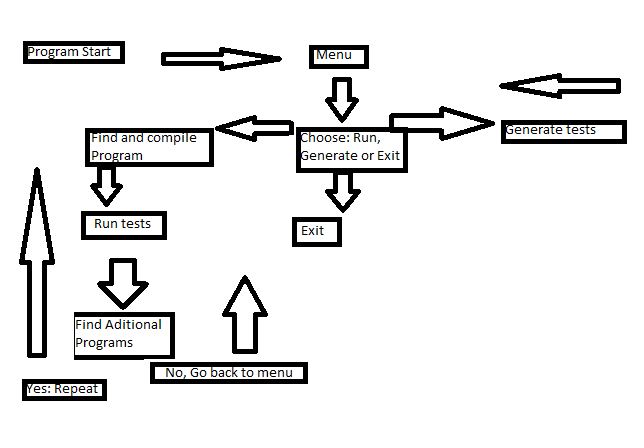
\includegraphics[width=0.75\textwidth]{./SystemDiagram}
\end{center}
\caption{System Diagram \label{systemdiagram}}
\end{figure}

\section{Technologies Overview}
The main programing langue used was C++, and was compiled with g++ on a linux environment.

% !TEX root = SystemTemplate.tex


\chapter{Project Overview}
This section provides information regarding the team and their roles,
how the project was managed, and any relatively unkown terminology or
acronyms.



\section{Team Members and Roles}
The team members were Erik Hattervig, the Product Owner; Andrew Koc, Tech Lead;
and Jonathan Tomes, Scrum Master.


\section{Project  Management Approach}

	The program was created through the Scrum Agile Approach.
The sprint length for this project was 2 weeks. We began with a meeting to
decide the user needs and split the program accordingly. Each of us would code
different parts of the program and then we would all test and re-code as needed.
placed on Trello to help design break points to split up the program between team members. 

	The code was stored, backed up, and shared through git hub. The back log and ownership 
was tracked through Trello. The user stories were condensed and 



\section{Phase  Overview}
Sprint 1 (Done by the team We Can't Follow Directions):

This program started in a gathering information phase, the first thing we had to do as a team 
was generate several questions to ask the customer (Dr. Logar) about the software that she 
wanted.   The next phase was asking if it could be done, as most of the code had been written 
at one point or another for our team, we decided that it was a program that could be written.  
The next phase was breaking the program into smaller milestones, we decided that the program 
would need to compile source code, search for test cases, run compiled code with test case, 
output test case results to a file, compare that output file to an expected output file, and then 
write to a file if the two files match or not, if they do we write the text case then passed to a log 
file, if they don't we write the text case and failed to the log file.   Once we are done traversing the 
directory we write the total number of passed, failed and percentages of each.

Sprint 2( Done by the team The Software Engineering Adventure Line):

First we began with an information gathering session by Dr. Logar and the product owners. This is where we
found out the goals of the program and the desired results. After this we were assigned a team's work
from the previous sprint, and evaluted it. Unfortunately we had to do a lot of revising and creating new
functions because the old cold was not very modular. So we divided up the work of reworking the code and
did our parts. After that we gathered and came up with how to meet the new requirements and worked out
what we needed to code, ask the user for, and finished coding the program.

\section{Terminology and Acronyms}
none

% !TEX root = SystemTemplate.tex
\chapter{User Stories, Backlog and Requirements}
\section{Overview}


This section will look at the userstories of the development of the program, the requirements
of the program, the proof o fconcept results, and research task results. It will also look at the
reason for developing this software. 

 The userstories 
Compile source code from tester.   Run compiled code from tester.   Compare two files from tester to see
if they are different.   Traverse a directory looking for test cases.   Write program output to a file.   Write
to human readable log file.   

Below:   list, describe, and define the requirements in this chapter.  
There could be any number of sub-sections to help provide the necessary level of 
detail. 





\subsection{Scope}


This document will contain stakeholder information, 
initial user stories, requirements, proof of concept results, and various research 
task results. 



\subsection{Purpose of the System}
To test a basic computer program written in the C++ language so a grade can quickly be assigned.


\section{ Stakeholder Information}


The person most interested in this project is Dr. Logar (the end user) who is looking to quickly, 
and easily, grade programs that are turned in by her CSC 150 students.   The people who want
to see us fail the most is our compitition (which Dr. Logar as graciously pointed out are our classmates 
on other teams). 


\subsection{Customer or End User (Product Owner)}
The product owner on the first sprint was Samuel Carroll, he created a list with his teammates 
and on a day, selected by Dr. Logar, met with her and the other teams' product owner to determine
exatly what Dr. Logar wanted. Samuel was also the team member most involved in keeping the Trello 
board up to date.


\subsection{Management or Instructor (Scrum Master)}
The scrum master for the first sprint was Colter Assman, his duties were to ensure that the project 
stayed on track and if any team member ran into some issues he would help them get back on track.   
Colter also was responsible for the running of the daily scrum.


\subsection{Investors}
There were no investors for our first sprint.


\subsection{Developers --Testers}
Shaun Gruenig was the biggest tester for our program.   As the team technical lead 
he kept us updated on if the project was running as we expected it to, and would 
often debug the issues our code had.


\section{Business Need}
Currently many computer science teachers have to write each test case out by hand.   
This is a very time consuming endeavor (especially considering how many students each
one has), so this program would enable them to write a test cases which will then be input
to our program.   Quickly and accurately giving grades to students.

\section{Requirements and Design Constraints}
The requirements was that our tester run in the Linux environment.   We also needed this 
program to be ready to send out by the time the first CSC 150 program was due, therefore
we only had about two weeks to write and implement this code.


\subsection{System  Requirements}
The program must be able to run on a Linux machine, using the GNU operating system.   
therefore the code must able to compile using the GNU compiler.   This means all of our
code must be executable on Linux machines.   Of course we may have had to write this
program for another system, but the Linux environment is the nicest one for us to use.


\subsection{Network Requirements}
No network requirements were needed.


\subsection{Development Environment Requirements}
Linux/GNU system should be able to run our tester. 


\subsection{Project  Management Methodology}
The stakeholders had several requests on how the project was implemented. Including 
what to use to keep track of backlogs and sprint status, which parties had access to the
sprint and produt backlogs, how many sprints will be used for this project, and restrictions
on the source control.
 
\begin{itemize}
\item Trello was used to keep track of the backlogs and sprint status
\item All parties will have access to the Sprint and Product Backlogs
\item Three sprints will encompass this project
\item The sprints will vary in length a little bit but be about 2-3 weeks in general
\item No specific source control is needed but we should familiarize ourselves with github
\end{itemize}

\section{User Stories}
This section contains information about the user stories (what the program must be able 
to do, and what the user should have to do).



\subsection{Compile and Run Source Code}
The program must be able to compile and run source code found in the directory

\subsection{Write Pass/Fail and Percentages to Log File} 
This program must be able to write output to a log file and to keep track of the total number
passed cases and the total number of failed cases.

\subsection{Compare Output with expected output}
The program must be able to compare the output that we get after running a test case to the
output that we expect to get from the test case. The expected output will be found when 
searching the directory.

\subsection{Searching/Traversing the Directory}
The program must be able to search through all the files and sub-directories of the directory 
that we are currently in.

\subsection{Invoking the Program}
The user must be able to run our program by typing `test <directory>'.


\section{Research or Proof of Concept Results}
Most of the code had been written by our team before.   We knew how to run the system 
function in C++ to invoke a system command. We had built a directory crawler in an earlier 
class (though in Windows so some modification had to take place).   All in all starting the 
program we knew we could complete it.


\section{Supporting Material}


In the man pages for the diff function it shows us that it returns one of three values and 
the case those values are returned, a zero if there is no difference between the two files, 
a one if there is a difference between the two files, or a two if something went wrong (doesn't happen often)


% !TEX root = SystemTemplate.tex
\chapter{Design  and Implementation}
This section will describe the design details for each of the major components 
in the system. 
 

\section{Parse Directory Function}

\subsection{Technologies  Used}
C++, Linux.

\subsection{Component  Overview}
This function will look for a C++ file, once it finds a C++ file it will compile it. 
This function will then call the find test, and run difference functions to run a test
and to see if there is a difference between the actual and expected outputs.

\subsection{Phase Overview}
This can traverse a directory, it can find and compile source code. It can look for, find, 
and run test cases. It can check for differences, and write to a log file.



\section{Find Test Function}

\subsection{Technologies  Used}
This will use C++ and system call function

\subsection{Component  Overview}
This function will travese a directory to find, and run test cases in our compiled 
source code. It will also write if the test case passed or failed, and increment our 
total count of passed and failed for the end of the log file.

\subsection{Phase Overview}
This function can traverse a directory looking for test case.  It can also run those 
test cases when it finds them, and write the results to the log file.  It also increments
the counter. 


\section{Run Difference Function}

\subsection{Technologies  Used}
This uses the C++, and system call function, as well as the diff function in Linux/GNU

\subsection{Component  Overview}
This function will create a function that will run the diff function in Linux/GNU via the system call.
First however it must create the string that will invoke the call, and take in the file names. Then it 
will pass inform others if the test case passed or failed so they can handle the information accourdingly. 
Also this doesn't print anything to the screen if there is a difference between the two files.

\subsection{Phase Overview}
This function can create the command string that will compare two files. This function will call the diff 
function. This function will not output anything to the screen if there is a difference between the two files. 
This function informs if there is, or is not, a difference between the two files.




% !TEX root = SystemTemplate.tex

\chapter{System  and Unit Testing}

The major testing used was running the program and trying to modify it to work how
we wanted it to.   The test cases provided by Dr. Logar provided a frame to base our
test cases on.

\section{Overview}
The first thing we did was get the code working.   Then we took the package provided to us
by Dr. Logar to see if the program was getting output that made sense. 



\section{Dependencies}
No testing framworks were used on this sprint.


\section{Test Setup and Execution}
The test cases were provided to us by Dr. Logar on the course website. 


% !TEX root = SystemTemplate.tex
\chapter{Development Environment}
This section will provide all the neccessary information to run, test and develop 
our source code.


\section{Development IDE and Tools}
The code was written in gedit and VIM, and requires no special IDE's or tools.

\section{Source  Control}
No source control system was used by our team for this sprint. We passed the code 
around through email, in future sprints we will need to start using a source control system.

\section{Dependencies}
The dependencies to building the system is our source code. 

\section{Build  Environment}
The packages are all built with the GNU compiler. There are no build scripts provided. 

\section{Development Machine Setup}
No special setup should be required to run our code.


% !TEX root = SystemTemplate.tex

\chapter{Release -- Setup -- Deployment}
The source code will be provided to Dr. Logar using email or the Submit It! page of
the SDSMT Math and Computer Science webpage.


\section{Deployment Information and Dependencies}
Will need g++ and a linux like environment to run our program.


\section{Setup Information}
By navigating to the directory and running make, the program will be installed.


\section{System  Versioning Information}
The system is in 2.0.0 stage, or second release.

% !TEX root = SystemTemplate.tex

\chapter{User Documentation}


%\newpage   %% 
%%  The user guide can be an external document which is included here if necessary ...
%%  a single source is the way to go.

\section{User Guide}

To use our program simply run it on the command line. You may specify a starting directory as a command
line argument, or the program will assume to run in the directory it already is in. Next a menu will apear
and ask for one of the options. 

Run will let the program run normaly, it will search through the directory
and find student directories containing the student source code. It will compile the code to the
root directory. It will then search through the test directory in the root to find test casses to run on the
student programs. It will log the result of each test to a student log file located in the student directory, and
the final result will be repeated in an overal class log located in the starting directory. If the student
fails a test labeled "crit\_(something).tst" the student will immediately fail and no more testing will be done.

Generate will then prompt for a number of test cases, the number of inputs per test, and finally a data type
to use for each test. It will then create a sub-directory called "Generated" in the test sub-directory of the root
where the program was prompted to go or started in. If it had previously created tests, it will clear the directory
and create a new one and all new test cases.

Exit will exit the program.


%% \newpage  %%  if needed ...
\section{Installation Guide}

1) Open the terminal and navigate to the directory containing our program source code and the makefile.

2) Run make.


%% \newpage  %%  if needed ...
\section{Programmer Manual}


% !TEX root = SystemTemplate.tex

\chapter{Class Index}
\section{Class List}
Here are the classes, structs, unions and interfaces with brief descriptions\-:\begin{DoxyCompactList}
\item\contentsline{section}{\hyperlink{class_poly}{Poly} }{\pageref{class_poly}}{}
\end{DoxyCompactList}






\backmatter
\chapter{Acknowledgement}
\label{SpecialThanks}  Thanks to Dr. Logar, and Shaun's Grandfather whom we named the
source code after  


\chapter{Supporting Materials}
There are, for this sprint, no supporting materials.


%%% Since counters are different in the backmatter section
%%% we explicitly set the section number  (comment out to see effect)
\setcounter{section}{0}
% !TEX root = SystemTemplate.tex

\chapter{Sprint Reports}

\section{Sprint Report \#1}
The testing function can traverse a directory looking for source code. Compile that code, then
look for test cases and run the compiled code with the given test case outputting the result in a 
new document. It can then compare that document with the expected results document and write
to the log file if it passed or failed. Then it will continue looking for test cases until all the test cases
in the root folder have been found. The tester will then write the total number of test cases passed,
total failed and the percentage passed and failed.

\section{Sprint Report \#2}

Had to redo a lot of the code. Most of it wasn't split into seperate functions and some of it was
misdocumented. After getting around that, we got it to travese the root directory, finding the
student directories and testing them against the tests located in the test directory. It can generate random
tests (the number of and data types specified by the user). Introduced a simple menu system to make it easier
to generate then run tests. It will log the results of the testing each student into a student log located in their
directory, and to a class log located in the root directory.

\section{Sprint Report \#3}

% !TEX root = SystemTemplate.tex

\chapter{Industrial Experience}

\section{Resumes}

%    \includepdf[pages={1}]{report.pdf}  %% example of limited page include

%     \includepdf{resume1.pdf}
%     \includepdf{resume2.pdf}
%     \includepdf{resume3.pdf}

\section{Industrial Experience Reports}

\subsection{Colter Assman}

% Report

\subsection{Samuel Carroll}

% Report

\subsection{Shaun Greunig}

% Report






\end{document}
